\chapter{Problem Search Test}
\label{chap:problem_search_test}
\myTop{In this chapter the test cases regarding the \cl{ProblemSearch} class and its methods: \me{Search} and \me{SearchSolvedFirst} are described.
It is generally the white box code coverage unit tests which are described in this chapter, because those are the most important, since we are focused on the functionality of our application and therefore want as much of our code tested as possible.}

\section{Unit Test Cases for the Search Function}
To test our problem search function, we have made an analysis of the code paths of the function.
The flow chart generated from this analysis is seen in figure \ref{fig:problem_search_flow}.
The decisions in the figure are labeled with a letter.
This is done because we want to refer to these decisions -- which are the conditions for loops to run another iteration -- later.
Notice that the loop labeled C is portrayed as a do-while even though code snippet \ref{src:search} shows that this loop is a while loop.
The reason for this is that the loop is a \verb|while(true)|, which breaks when an exception of the type \cl{NotSupportedException} is thrown.
This means that the loop will always run at least once, like a do-while loop.
This is more thoroughly described in subsection \ref{sub:searchTags}.

To make test cases a set of tags and problems are needed to test upon.
These are seen in figure \ref{tab:problem_search_base}.

\begin{figure}[hp]
	\centering
		\begin{tabular}{|c|c|c|c|c|c|}
		\hline
			Problem	& \multicolumn{4}{c|}{Tag} & Solved \\ \hline
								& 0&1&2&3& \\ \hline
			0					& $\checkmark$ & $\checkmark$ & & & \\ \hline
			1					& $\checkmark$ & $\checkmark$ & & & $\checkmark$  \\ \hline
			2					& & & & & \\ \hline
			3					& $\checkmark$& & & & \\ \hline
			4					& & $\checkmark$& & & $\checkmark$ \\ \hline
			5					& & & & $\checkmark$ & \\ \hline
		\end{tabular}
	\morscaption{The problems and tags which the test cases are based upon}
	\label{tab:problem_search_base}
\end{figure}

\label{sec:unit_problem_search}
\begin{figure}[p]
	\centering
		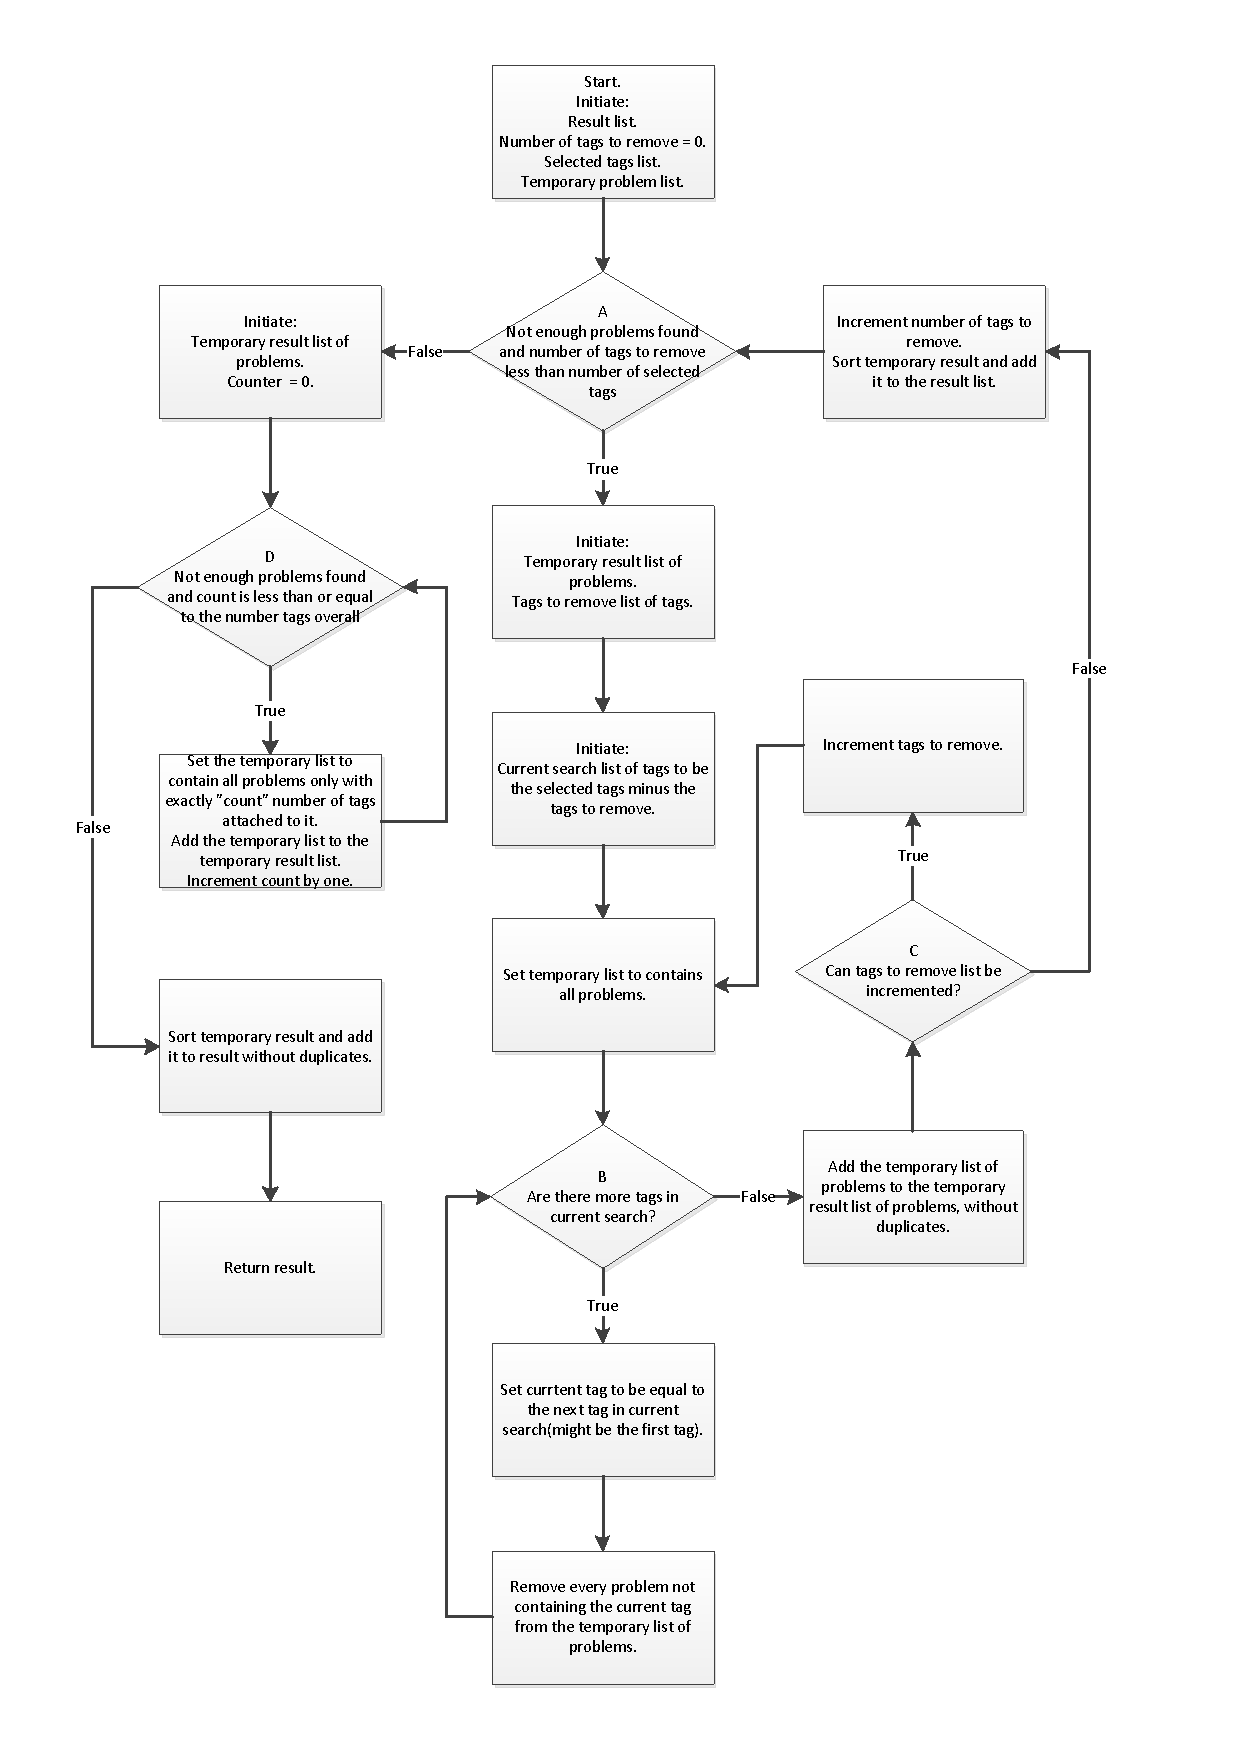
\includegraphics[width=1.25\textwidth]{input/testing/problem_search.pdf}
	\morscaption{Flow chart of the search function.
	The letters in the decisions indicates which loop they are associated with, e.g. the decision labeled A is associated with the loop A}
	\label{fig:problem_search_flow}
\end{figure}


\subsection{Test Case One}\
\begin{lstlisting}[style=sourceCode, caption=\myCaption{The test case for no run of any loops}, label=src:noLoops,float=htb]
#region Test 1: Search for no tag, minimum number of problems = 0
[TestMethod()]
public void A0_D0_SearchForNoTagNoProblems()
{
	#region Arrange
	List<Problem> expected = null;
	List<Problem> actual = null;
	int minNoProb = 0;

	expected = new List<Problem>();
	#endregion

	#region Act
	actual = ProblemSearch.Search(catTag,
		problems, tags, minNoProb);
	#endregion

	#region Assertions
	Assert.AreEqual(expected.Count, actual.Count);
	#endregion
}
#endregion
\end{lstlisting}

Since the search method only contain loops and no if statements, the focus for the test cases regarding the search is on the loops edge conditions.
The first test case will test the option where none of the loops are run.
If \textit{A} is not run, \textit{B} and \textit{C} will never be run because they are inside of the \textit{A} loop.
\textit{A} will not be run if either the size of the result is at least equal to the minimum number of problems to find or if the number of tags to remove is at least equal to the number of selected tags.
To not run the \textit{A} loop, the number of selected tags is set to 0, i.e. no tags are selected.
The \textit{D} loop will not be run if enough problems are found or if the \vari{count} variable is higher than the number of all tags.
Because of this the minimum number of problems to find is set to zero.
This test case is seen in code snippet \ref{src:noLoops}.
The \cl{ProblemSearch} is the class which which is being tested in the code snippet, particularly the \me{Search} method in this test case.

\subsection{Test Case Two}
The next test case will test the same as the above test case, except for the fact that the \textit{D} loop will run exactly once instead of zero times.
This time the minimum number of problems to find is set to one, while keeping all other input the same as the previous test.
This will result in the \textit{A} loop not to run and the \textit{D} loop to run exactly once, because it would then find problem number two, which is the only problem with no tags attached.. As seen on figure \ref{tab:problem_search_base}.
The source code for this test case is shown in appendix \ref{chap:problem_search_test_source}.

\subsection{Test Case Three}
This test case should not run loop \textit{A}, but run loop \textit{D} more than once.
This is accomplished by increasing the minimum number of problems to find to 6 while keeping the number of tags to be zero.
This test case is shown in appendix \ref{chap:problem_search_test_source}.

\subsection{Test Cases Four to Six}
Now that we have tested all code paths not containing any runs of the \textit{A} loop, the next test cases will consider the cases where \textit{A} is run once.
To run loop \textit{A} once, there most be a positive number of tags selected.
If the \textit{A} loop is run then both the \textit{B} and \textit{C} will be run at least once, for the following reasons:
\begin{itemize}
	\item \textit{B} will be run because the first time the current search is initialized, it will contain all selected tags, which must be at least one, therefore the \textit{B} decision in figure \ref{fig:problem_search_flow} will render true at least once and run the \textit{B} loop.
	\item As described earlier the \textit{C} loop acts as a do-while loop for reasons explained earlier in this section, thereby allowing the \textit{C} loop to be run at least once.
\end{itemize}

For test case four the \textit{A}, \textit{B}, and \textit{C} loop will be run one time and the \textit{D} loop zero times.
Test case five will allow \textit{D} to be run exactly one time, and test case six will let \textit{D} run several times.
All the test cases can be seen in appendix \ref{chap:problem_search_test_source}.
To vary the number of times which \textit{D} is run, the minimum number of problems to find is simply raised while the number tags selected remains one in order for the loops \textit{A}, \textit{B}, and \textit{C} to run only a single iteration each.

\subsection{Test Cases Seven to Nine}
The test cases should run loop \textit{A} multiple times and change the number of runs the loops \textit{B}, \textit{C}, and \textit{D} runs.
As shown above the  number of times loops \textit{A} and \textit{D} runs can be changed independently.
The number of iterations that the number \textit{B} and \textit{C} loops will take is however very dependent on the number of times \textit{A} will run.
For \textit{A} to run more than once, the number of selected tags most be more than one and the number of problems found in the first run of loop \textit{A} must not exceed the minimum number of problems to find.
At the first run of \textit{A} the \textit{B} loop will run $x$ times, where $x$ is the number of selected tags.
Because the current search during the first iteration of \textit{A} will contain every selected tag, which is more than one, thereby letting \textit{B} run more than one time.
During the second run of the \textit{A} loop, the \textit{C} loop will run $x$ times, where $x$ is the number of selected tags.
The reason for this is that the search will be ``softened'' and only search for problems with all but a specific tag in each iteration, which will render searches in which a different tag is missing each time. 

The three test cases which will cover the last code paths are:
\begin{itemize}
	\item The \textit{A}, \textit{B}, and \textit{C} loops are run several time and the \textit{D} loop is run zero times.
	\item The \textit{A}, \textit{B}, and \textit{C} loops are run several time and the \textit{D} loop is run exactly once.
	\item The \textit{A}, \textit{B}, \textit{C}, and \textit{D} loops are run several time.
\end{itemize}
To ensure that the \textit{A}, \textit{B}, and \textit{C} loops are run more than once, the number of selected tags is set to two and the minimum number of problems to find is set appropriately.
The test cases are shown in appendix \ref{chap:problem_search_test_source}.

\subsection{Regression Test Cases}
\label{sec:regression_problem_search}
The same test cases as described above are used as regression test cases, to ensure that no new change will sabotage any of the already working code.
There could be made a new analysis of the code each time a change is made, but this will take a lot of time, and will not necessarily generate better test cases.
\myTail{This chapter describes the test cases used to test the \me{Search} method belonging to the \cl{ProblemSearch} class.
Beside the code snippet in this chapter, the appendix \ref{chap:problem_search_test_source} holds the source code for the described unit tests.}